\documentclass[a4paper, norsk, 10pt]{article} % Define document type and size
%% LaTeX Preamble - Common packages

\usepackage{array, xcolor} % Table packages
\usepackage{url} %Package for formating url properly use \url{www.example.com}


%% Three packages for handling norwegian symbols
\usepackage[utf8]{inputenc}
\usepackage[norsk]{babel}
\usepackage[T1]{fontenc}


\usepackage{graphicx} % Package for handling figures and pictures
\usepackage{caption}
\usepackage{subcaption} % Package for handling captions
\usepackage{calc} % LaTeX calculates for instance width from algebraic expressions
\usepackage{enumitem} % List woth numbers
\usepackage{longtable}

\setlength{\voffset}{-45pt}
\setlength{\textheight}{730pt}
\setlength{\topmargin}{-5pt}
\setlength{\headsep}{0pt}
\setlength{\textwidth}{500pt}
\setlength{\hoffset}{-70pt}
\usepackage{hyperref}
\hypersetup{
    colorlinks = true,
    linkbordercolor = {white},
    allcolors = cyan
}
\usepackage[autostyle]{csquotes}

%%%%
%% DEFINE TABLE SETTINGS
%%%%
\definecolor{lightgray}{gray}{0.8}
\newcolumntype{L}{>
{\raggedleft}p{0.16\textwidth}} % 0.14
\newcolumntype{R}{p{0.84\textwidth - 4\tabcolsep}} % subtract off 4 times \tabcolsep

\newcommand\VRule{\color{cyan}\vrule width 0.42pt}

\title{}
\author{}
\date{}


\begin{document}
\pagenumbering{gobble} % Remove pagenumbering

%%%%
%% INSERT PICTURE
%%%%
\begin{figure}[h]
\begin{subfigure}[b]{2.6cm}
\fboxrule=0.2pt%border thickness
\fboxsep=0.9mm%padding thickness
\fcolorbox{cyan}{white}{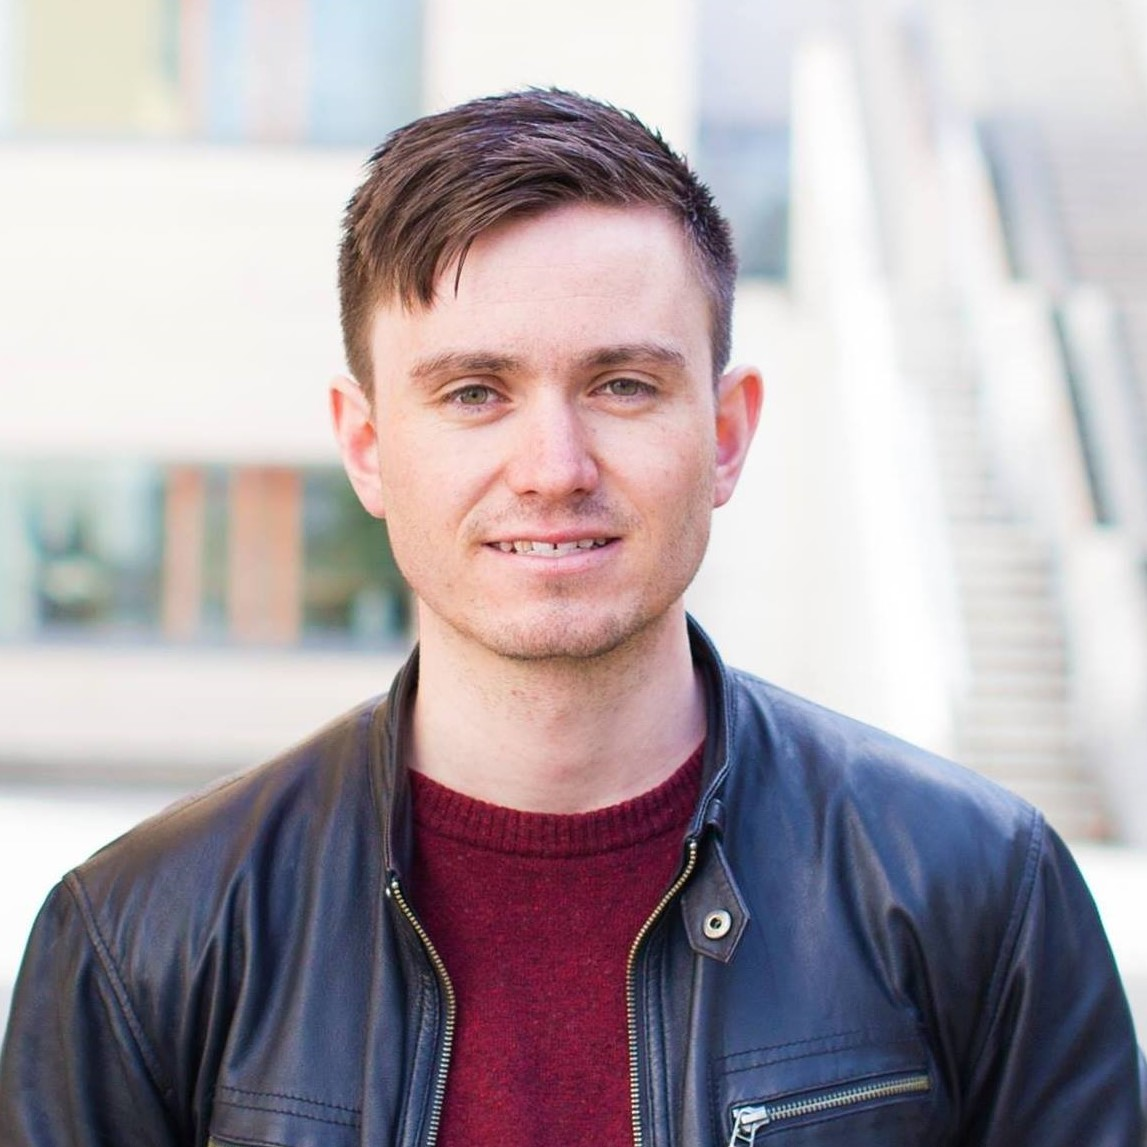
\includegraphics[scale = 0.064]{bilde_1.jpg}}
\end{subfigure}
\begin{subfigure}[b]{9cm}
   	\textsc{\bfseries{\Huge{Thomas Kleiven}}} \\[5pt]
   	\textsc{\Large{Ingeniørvitenskap \& IKT}} \\[5pt]
   	\textsc{\Large{Curriculum Vitae}}
\end{subfigure}
\end{figure}

%%%%
%% INSERT ADDRESS AND CONTACT INFORMATION
%%%%
\begin{table}[h]
\noindent \begin{tabular*}{\textwidth}{@{\extracolsep{\fill}} l r}
Edgar B. Schieldropsvei 100B & 19. Juni 1994 \\
7033 Trondheim & 
\includegraphics[scale=0.042]{phone.png}  +47 930 47 147\\
Norge
 & 
\includegraphics[scale=0.013]{mail.png} \href{mailto:thomas@isvik.no}{{thomas@isvik.no}} \\
 & 
\includegraphics[scale=0.020, trim={2mm 28mm 2mm 2mm}, clip]{linkedin_logo.png} \href{https://no.linkedin.com/in/thomaskleiven}{{thomaskleiven}} \\
 & 
\includegraphics[scale=0.013, trim={0mm 0mm 75mm 0mm}, clip]{github.png} \href{https://github.com/thomaskleiven}{{thomaskleiven}}
\end{tabular*}
\end{table}

%%%%
%% WRITE SUMMARY. VURDER SELV OM DU VIL HA DETTE AVSNITTET
%%%%
%%\section*{Summary}
%%\begin{itemize}[noitemsep, nolistsep]
%%\item Broad laboratory experience, especially within cell and molecular biology. Know the importance of being thorough and organized and the value of good lab practice.
%%\item Experience with administrative procedures, budget planning and organizing meetings and conferences.
%%\item Experience with MS Office, \LaTeX and HTML and basic skills in programming (Python).
%%\item Great communication and organizational skills.
%%\item Technically minded and with good problem resolution skills. Willing to learn new skills and able to pick up new tasks quickly.
%%\item Able to work effectively in fast paced and ever changing environments.
%%\item Currently taking french lessons.
%%\item Interested in both administrative and laboratory work %%tasks.
%%\end{itemize}*%


%% Dette avsnittet er kanskje mest relevant for dersom du har spesiell laberfraing
%%\section*{Technical Skills}
%%\begin{tabular}{L!{\VRule}R}
%%Molecular Biology & Transformation, plasmid preparation, PCR, gel electrophoresis, DNA cloning techniques, DNA isolation and extraction \\
%%Cell Biology & Prepare media, making LB solution and agar plates, aseptic techniques, streak plating, human cell cultivation\\
%%Organic chemistry & Chromatography, mass spectrometry (LC-MS) \\
%%Bioinformatics & Pub Med, Blast NBCI, Clone Manager, Psipred, ChemDraw \\
%%\end{tabular}

\section*{Utdanning}
\begin{tabular}{L!{\VRule}R}
2014 - & {\bf Sivilingeniør/Master i Ingeniørvitenskap og IKT, {NTNU Gløshaugen}, \normalfont{\textit{Trondheim}}} \\
  & {Spesialisering innen Produksjonsledelse \& IKT. Hovedprofilen 		fokuserer på utvikling av IKT-systemer for integrasjon av operasjoner i bedrifter og i globale verdikjeder, i tillegg til å bygge bro mellom datatekniske og ingeniørfaglige utfordringer.} \\
\vspace*{0.001pt}2013 - 2014 & {\bf \vspace*{0.001pt} Førstegangstjeneste, Hans Majestets Kongens Garde, \normalfont{\textit{Oslo}}} \\
    &{Drillgardist i HMKG Drilltropp. Gjennomførte oppdrag i inn- og utland, i tillegg til å ta eksamen i emnene `Jus og Militærmakt' og `Etikk og Militærmakt'.} \\
\vspace*{0.001pt}2010 - 2013 & {\bf \vspace*{0.001pt} Videregående skole, Skeisvang vgs, \normalfont{\textit{Haugesund}}}  \\
\end{tabular}

\section*{Arbeidserfaring}
\begin{tabular}{L!{\VRule}R}
2016 & {\bf Summer Intern, {Statoil ASA}, \normalfont{\textit{Kårstø}}}
\\
& Bisto operatører på anlegget, i tillegg til å lage en applikasjon for å kunne sammenligne lokale og globale momentverdier. Implementerte algoritmen i Java, og brukte JavaFX \\&til GUI.  \\
\vspace*{0.001pt}2013 - 2015 & {\bf \vspace*{0.001pt}Sommerjobb, {Møbelringen Math. Lande AS}, \normalfont{\textit{Haugesund}}} \\
& Sommerjobb - Utkjøring og montering av møbler, kundebehandling og lagerarbeid \\
\vspace*{0.001pt}2008 - 2012 & {\bf \vspace*{0.001pt}Deltidsjobb som Vedlikeholdsansvarlig,{ Isvik Helse AS}, \normalfont{\textit{{Vindafjord}}}} \\
& Diverse vedlikeholdsoppgaver og renhold  \\
\end{tabular}


\section*{Dataferdigheter}
\begin{tabular}{L!{\VRule}R}
 OS & \textsc{Windows, Macintosh, Linux} \\
Programmering & \textsc{MATLAB, Java, Python, C++}\\
Tekstbehandling & \textsc{MS Office, \LaTeX}\\
Versjonskontroll & \textsc{Git}\\
PLM Software & \textsc{Siemens NX} \\
ERP Systemer & \textsc{SAP, Microsoft Dynamics AX}
\end{tabular}

\section*{Frivillig verv}
\begin{tabular}{L!{\VRule}R}
2015 - 2017 & {\bf Styreleder, {NTNUI Triatlon}, \normalfont{\textit{Trondheim}}} \\
&  Ansvarlig for klubbens adiminstrative del. Hovedansvar for flere arrangement i klubbens regi, deriblant Norges første studentmesterskap i triatlon. I løpet av de siste to årene har klubben doblet antall medlemmer, og vi er nå mer enn 70 medlemmer.\\

\end{tabular}

\section*{Språk}
\begin{tabular}{L!{\VRule}R}
Norsk & Morsmål \\
Engelsk &  Flytende skriftlig og muntlig \\
Tysk & God skriftlig og muntlig \\
\end{tabular}


%%\section*{Referanser}
%%\begin{tabular}{L!{\VRule}R}
%%1.  & Roy Høystad, Daglig leder Møbelringen Math Lande AS, Haugesund  \\
%%& roy.hoystad@mml.no \\
%%& +47 481 68 305 \\
%%2.  & Even Kallevik, Økonomiansvarlig NTNUI Triatlon\\
%%& triatlon-kasserer@ntnui.no \\
%%& +47 902 44 868 \\

%%\end{tabular}

%\section*{Vedlegg}





\end{document}
